\section{MATRIX}

Matrix is an open protocol for decentralised communication. It aims to make 
communication platforms interoperable and federated.

The main idea is to make real-time communication work seamlessly between different chat 
service providers, allowing users with accounts at one communications service provider to 
easily communicate with users of a different service provider.

Users have the privilege to communicate with people outside the Matrix network through bridges, 
which connect previously established communication networks, such as Slack and IRC, to the Matrix network.
With bridges, the need for using different apps to talk to different people is eliminated. Whatever Matrix 
client the user chooses, can talk to anyone inside or outside the Matrix network.

Matrix gives users total control over their communication by letting them run or select their own 
server while still participating in a global network, rather than being locked in silos 
like Signal, WhatsApp, Telegram, Slack etc. 

The key feature of Matrix is that no single server hosts or controls a given conversation -- instead, 
as one user communicates with another, the conversation gets replicated equally across the servers -- meaning 
all the participants equally share ownership over the conversation and its history. 
There is never a central point of control or authority, 
unless everyone decides to use the same server.~\cite{MATRIXorgOpenProtocol}

By default, Matrix uses simple HTTPS+JSON APIs as its baseline transport, but also embraces 
more sophisticated transports such as WebSockets or ultra-low bandwidth Matric via CoAP+Noise.~\cite{MATRIX}

Applications using the Matrix protocol, called Matrix clients, have all the features one would
want and expect from a modern chat app: instant messaging, group chats, audio and video calls, 
searchable message history, synchronization across all devices, as well as end to end encryption.
Element is the best known Matrix client.
Via Matrix, Element is able to bridge communications like IRC, Slack and Telegram into the app.~\cite{RumaMATRIX}

\begin{figure}[h]
    \begin{center}
        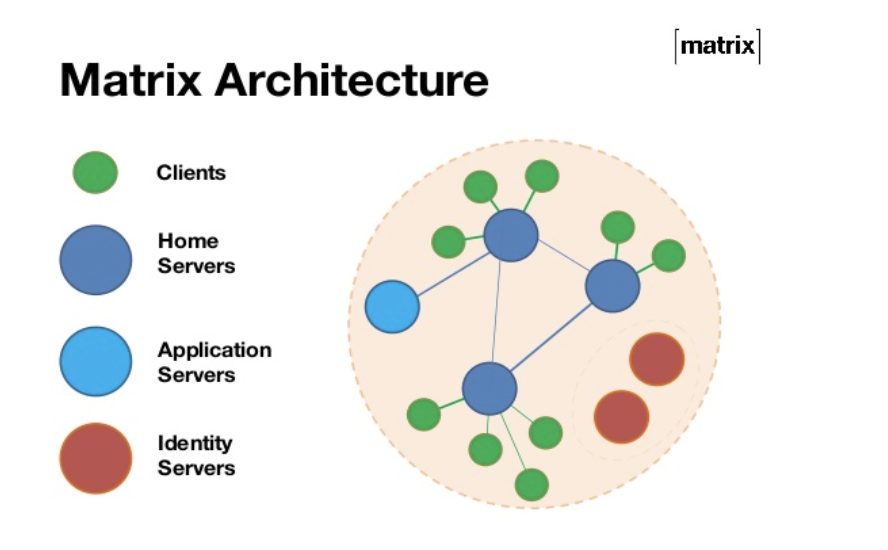
\includegraphics[width=10cm]{matrix.png}
    \end{center}
    \caption{An example of a Matrix Architecture, illustrated very simply using abstract coloring.}
    \label{fig:matrix}
\end{figure}

\subsection{Conclusion}

As a result of several chat services not being interoperable with each other, people are 
forced to use multiple services to communicate.
However, since Matrix is federated, just like email, the sender can freely communicate across a 
global network, without having to use specific services based on which ones the intended receiver uses.

Another major problem with online communication today is that most of the services 
are operated by commercial organizations. This means the user's data is only protected by policy, and not by design.
But because Matrix is federated, the user has control over their data storage and access.~\cite{RumaWhyMatrix}
